%% \documentclass[10pt]{article}
%% \documentclass[10pt,technote]{IEEEtran}
\documentclass[conference]{IEEEtran}

\usepackage[skip=7pt plus1pt, indent=0pt]{parskip}
\usepackage{hyperref}
\usepackage[margin=1.0in]{geometry}
\usepackage{cite}
\usepackage{graphicx}
\usepackage{caption}
\usepackage{subcaption}

\newcommand{\tall}{\phantom{\large QqK}}
\newcommand{\mAP}{m\textsc{AP} }

\IEEEoverridecommandlockouts

\AtBeginDocument{%
  \providecommand\BibTeX{{%
    Bib\TeX}}}

\begin{document}

\title{\textsc{CMPE-256}: Million Song Dataset Challenge$^\star$}
\date{}


\author{
\IEEEauthorblockN{Carlos Hernandez}
\IEEEauthorblockA{
\textit{Computer Engineering Dept.} \\
\textit{San Jose State University} \\
{\small \texttt{carlos.hernandez@sjsu.edu}}}
\and 
\IEEEauthorblockN{Hardy Leung\thanks{${}^\star$ 
\texttt{https://github.com/jfantab/cmpe256-project}}${}^\star$}
\IEEEauthorblockA{
\textit{Computer Engineering Dept.} \\
\textit{San Jose State University} \\
{\small \texttt{kwok-shing.leung@sjsu.edu}}}
\and 
\IEEEauthorblockN{John Lu}
\IEEEauthorblockA{
\textit{Computer Engineering Dept.} \\
\textit{San Jose State University} \\
{\small \texttt{john.lu@sjsu.edu}}}
}

\maketitle

\begin{abstract}
We sought to investigate the Million Song Dataset (MSD)
\cite{Bertin-Mahieux2011}, an anonymized collection of user data and metadata
for popular contemporary songs. In the accompanying Kaggle MSD Challenge
(MSDC), over 150
teams proposed solutions to predict which songs a user will listen
to, given the collective listening history of all users.
The sizable training data contains over 1M listeners, 380K songs,
and 48M user-song-play triplets.
In this project,
we studied multiple collaborative filtering techniques; our best
result of 17.453\% would have placed us in the second place in the Kaggle
Challenge.
\end{abstract}

\begin{IEEEkeywords}
recommender system, implicit feedback
\end{IEEEkeywords}

\section{Introduction}

The Million Song Dataset (MSD) is
a collection of user data and metadata for popular contemporary songs.
MSD was designed to encourage research on algorithms that scale to commercial sizes,
and to provide a reference dataset for evaluating research \cite{Bertin-Mahieux2011}.
Most relevant to
our project is the taste profile of over $1M$ listeners, captured in $48M$
user-song-play triplets. While users are fully anonymized, MSD provides a rich collection
of information related to the songs, including
genre classification from the Tagraum dataset \cite{schreiber2015improving},
the MusiXmatch lyrics dataset \cite{Bertin-Mahieux2011},
and even acoustic and spectral analysis. In its
entirety, the MSD contains a total of 280GB worth of data
\cite{Bertin-Mahieux2011}.

In the MSD Challenge, each of the $48M$ user-song-plays triplets is a positive integer 
representing the number of times a user has played a specific song. While we will adopt
familiar terminologies as item-based (IB) and user-based (UB)
collaborative filtering, and matrix factorization (MF), we are
nonetheless making recommendations based on {\em implicit} feedback, where
the non-zero entries in the utility matrix should be
interpreted as merely a signal, rather than a definite opinion or rating.

\section{Related Work}

The Netflix Prize competition that began in 2006 was a key
driving force behind the rapid
adoption of many collaborative filtering techniques across high-tech
industries \cite{bennett2007netflix}, such as
the popularization of matrix factorization by Simon Funk in his tongue-in-cheek blog post
\cite{funk2006try}. However, it is rare to find datasets that employ explicit
ratings in real-life.
More frequently, the feedback would come implicitly in the form of a click, a listen, a purchase, and
so on. While a positive feedback does signal preference, an absence of feedback should not be interpreted as a definitive negative opinion. In \cite{hu2008collaborative}, Hu et al.~adopted a
formulation where implicit feedbacks are coupled with {\em confidence}, modeled as larger
weights in the objective function; they also made a clever and necessary adaptation of the
Alternating Least Square (ALS) algorithm to handle the dense
loss function induced by their formulation,
where even empty terms receive a non-zero, albeit diminutive, penality.
Subsequently, Johnson \cite{johnson2014logistic} extended
Hu's work with a logistic formulation that directly models the 
probability that a user will prefer a specific item.

In the MSD Challenge, the objective is to predict the song preference of
each of the $110K$ users in the testset, given half of
their song preference, and the complete listening history
of $1M$ users in the trainset.
We were to offer an individualized and ranked list of
$\tau$ recommended
songs to each of those users, where $\tau = 500$ in the MSD
Challenge.
The prediction is then measured with the truncated
\mAP metric. We first need to define
$precision\textrm{@}k$ to be the fraction of correctly predicted songs
within the first $k$ recommendations. Then, the truncated \mAP metric
evaluates $precision\textrm{@}k$ at each rank with a correct prediction,
divided by the number of the hidden songs (correctly predicted or not).
For example, if a user $u$ has $5$ hidden songs,
$3$ of which were ranked within the $500$ predictions at $3^{\rm rd}$,
$7^{\rm th}$,
and $20^{\rm th}$ places, and the remaining two were not predicted at all.
Then, the truncated
\mAP for the user is:

\hspace{1em}$\frac{1}{5}\left(\frac{1}{3} + \frac{2}{7} + \frac{3}{20}
\right) \simeq 0.15381$

This example shows that we can achieve a higher \mAP score by correctly
predicting more songs at higher ranks.
%% Keep in mind that there are over $380K$ songs in the dataset,
%% and the average user in the testset only has $25$ hidden songs. It is
%% extremely to correctly predict the songs.
%% it is 
%% a random prediction of 
%% and the chance of correctly
%% predicting {\em any} of the hidden songs (averaging $25$ per user in the
%% testset) is abysmal. We shall revisit this issue in the discussion section.

\section{Our Approach}

Armed with a good understanding of what the project entails,
we set out to experiment with the following techniques, each of which
was carefully considered beyond simple application of existing packages.

\begin{itemize}
\item algorithm design and architecture engineering
\item neighborhood-based collaborative filtering
\item matrix factorization for implicit feedback
\item similiarity based on factorized latents
\item similiarity based on embeddings of metadata
\item term-frequency document-frequency normalization
\item ensemble recommendation
\end{itemize}

\subsection{Algorithm Design and Architecture Engineering}

A crucial decision was made to develop the program using C++, and most
of the experiments were run on a modestly equipped laptop.
We did evaluate a few options, including HPC, Google CoLab,
and various Python and Java packages. At the end, we decided that having a
flexible and properly engineered architecture is just as important as
choosing the right algorithms,
even more so if the algorithms were designed with
the architecture in mind. The C++ code was written completely from scratch,
with the exception of a small JSON parser, and thus we avoided significant
amount of external dependencies, such as GPU availability and
reliability, timeout issues with cloud-based
computing, and lack of transparency in implementation characteristics
of gray-box packages.
We engineered the algorithms
to take full advantage of multi-threaded parallelism, and to fit under
approximately $4$GB of RAM to avoid disk thrashing. While this was an
old-school approach to engineering and optimization, doing so allowed us
to run various algorithms in a reasonable amount of time.
We did
make multiple design tradeoffs given several
naïve
implementations would have required
$O(|U|\times |I|)$, $O(|U|^2)$, or $O(|I|^2)$
memory, where $U$ is the set of users, and $I$ is the set of
songs. Since $|U| \simeq 1.1M$ and $|I| \simeq 380K$, those implementations
would have simply run out of memory.

Our basic architecture is simple yet designed with performance in mind.
The utility matrix $M$ is implemented as two complementary matrices
called \textsc{uir} and \textsc{iur} (which stand for User-Item-Rating
and Item-User-Rating), implemented as indexed arrays to afford
$O(1)$ lookup of both $I_u$ (all items rated by the user $u$) and $U_i$
(all users who rated the item $i$). \textsc{uir} is sorted first by $U$ and then
by $I$, whereas \textsc{iur} is sorted first by $I$ and then $U$. This allows
us to enumerate the set $U_i$ in increasing order of user, and similarly for
$I_u$.
The memory requirements of \textsc{uir} and
\textsc{iur} are both $|M|$. In our case,
$|M| \simeq 48$ million.
Note that $\sum_{u\in U} |I_u| = \sum_{i\in I} |U_i| = |M|$.

The simplest approaches to solving MSD would be the familiar user-based
(UB) and item-based (IB) collaborative filtering, which we implemented first
as a baseline, and then carefully extended. 
Note that
the number of plays should not be used as rating, since it is both
unreliable and unbounded. Moreover, since our goal is to predict
{\em whether} a user would play a song, it makes sense to binarize the
utility matrix $M$ so that an entry is $1$ if
the user played the song at least once, and $0$ otherwise.
In the following, we assume $M$ has been binarized unless stated otherwise.

While UB and IB are conceptually simple, we have two serious problems.
First, $U$ and $I$ are both very large. Second,
we need to make a total of $|U_{\rm test}|
\times |I|$ predictions,
where $U_{\rm test}$ is the subset of users to receive
our top-$500$ recommendations\footnote{
To put things in perspective, $|U_{\rm test}| \times |I| = 42$ trillion,
but the Netflix Prize only asked for $2.8$ million predictions.}.
%% Each of these $42$ trillion entries,
%% if evaluated separately, could also be extremely expensive.
In IB, we'll look at each item $i \in I_u$, and
compute $sim(i, j)$, defined to be the similarity score between items $i$
and $j$. Even worse, $sim(i, j)$, if again evaluated individually,
would require going through both $U_i$ and $U_j$, taking at least
$O(|U_i| + |U_j|)$ time. All these add up to a serious complexity problem.

This problem is not unique to us. In fact, the Python Surprise
package \cite{hug2020surprise}
precomputes an $O(|I|^2)$ array of $sim(i, j)$, since
we need to access the value of $sim(i, j)$ very frequently. The problem is
that $O(|I|^2)$ is a very large number ($\simeq 144$ trillion entries in
our case), and 
Surprise would quickly run out of memory. Clearly, we need
a different approach.

We still want to compute all $|I|^2$ pairs of $sim(i,j)$, and we process
each item $i$ one at a time, but all $sim(i,\star)$ would be
computed simultaneously. To address the memory problem, 
for each item $i$, we would keep at most $K$ best (i.e.~largest)
$sim(i,j)$. 

For each $i$, we first initialize a $count(i,\star)$ array
to zero, and go through each user $u \in U_i$, and for each
item $j$ in $I_u$, we simply increment $count(i,j)$. This simple
sequential pass allows us to count, for each $j$,
the number of users who played both $i$ and $j$ (keep in mind that we are
working on a particular item $i$).
Next, we turn $count(i,\star)$ into $sim(i,\star)$
with a straight-forward formula in $O(1)$ time.
Finally, we will
find the collection of $K$ largest $sim(i,\star)$ using
a linear-time median-finding algorithm\footnote{
We used \texttt{std::nth\_element()}, which
found not only the $n^{th}$ element, but all elements smaller than said
element. This is done in linear time in the size of the vector.}, and we
store the result into an array of size $K$.
In our implementation, we set $K = 500$.

Together, computing all $sim(i,\star)$ takes $(|I| + |M_{U_i}|)$ time, where
$M_{U_i}$ is the subset of the utility matrix $M$ taking only rows
corresponding to users in $U_i$. Summing over all possible $i$,
the total runtime complexity of our
IB implementation is:

\hspace{1em}$\sum_{i\in I} O(|I| + |M_{U_i}|) = O(|I|^2) + O(\sum_{i\in I}|M_{U_i}|)$

which can be rewritten as:

\hspace{1em}$O(|I|^2) + O(\sum_{u\in U}|I_u|^2) = O(|I|^2 + \beta_{\rm item}^{\rm M} |M|)$

where $\beta_{\rm item}^{\rm M}$ is a (non-constant) multiplier determined by the characteristics of
the matrix $M$. It is as if
we would process all items of user $u$, namely $I_u$, exactly $|I_u|$ times.
This does imply a quadratic behavior, albeit on a per-user basis.
Empirically, $\beta_{\rm item}^{\rm M} = 118$.
Note that $\beta_{\rm item}^{\rm M} = O(|I|)$ but in practice
$\beta_{\rm item}^{\rm M}$ is likely significantly
smaller than $|I|$ (by $3200X$).

Let $sim^K(i,j)$ denote the abridged version of $sim(i,j)$,
where only the best $K$ entries of $sim(i,\star)$ are kept for each $i$.
The memory requirement is therefore
$O(K|I|)$ for IB and similarly $O(K|U|)$ for UB.
In our case, given $K=500$, they amount to $190M$ and $555M$ entries 
respectively for IB and UB collaborative filtering. We can further improve
the memory footprint by reducing $K$, but the entirety of
$sim^K(i,j)$ needs to be
kept in memory for downstream usage.
We did perform a cursory analysis on the impact of reducing
$K$ on the performance of our IB recommender,
as shown in Figure \ref{fig:log2k} (note that the $x$-axis is on a
logarithmic scale, and $500 \simeq 2^9$). It seems reducing $K$ to
$64 = 2^6$ or even $32 = 2^5$ has negligible impact on performance.

\begin{figure}[htbp]
\centering
\begin{subfigure}{0.85\columnwidth}
  \centering
  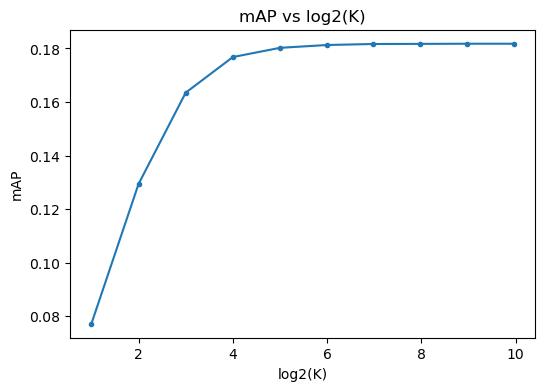
\includegraphics[width=\columnwidth]{log2k.png}
\end{subfigure}
\caption{The \mAP performance of an IB run with different values of
$K$, where $K$ is the maximum number of $sim(i,\star)$ kept in
memory for each item $i$.}
\label{fig:log2k}
\end{figure}

Once we conclude the computation of $sim^K(i,j)$, we perform recommendation
for each user, starting by initializing a score array of size $|I|$ to
zero. $rec(u,i)$ represents the prediction (or recommendation)
of item $i$ to user $u$. We will go
through each item $i$ in $I_u$, retrieving all $K$ items in
$sim^K(i,\star)$, and increment $rec(u,j)$ as follows:
\begin{eqnarray*}
rec(u,j) \leftarrow rec(u,j) + \left(r_{u,i}\right)\left(sim(i,j)\right)
\end{eqnarray*}
for each eligible $j \in sim^K(i,\star)$. In essence, we concurrently
update all $rec(u,\star)$.
The update per user takes $O(K\times |I_u|)$ time, and thus
in aggregate the complexity for all $U_{\rm test}$ users is
$O(K\times |M_{\rm test}|)$.
Since $K=500$ and $|M_{\rm test}| \simeq 0.1\times |M|$, it would be
similar to going through the utility matrix $M$ $50$ times.

Note that the computation of both $sim(i,j)$ and $rec(u,i)$ can be
parallelized. We decided that a multi-threaded approach would perform best,
and in fact were able to achieve near linear speedup,
close to $750\%$
CPU utilization with a hyperthreaded Quad-Core CPU.
To reiterative, the runtime complexity of our
IB implementation is:

\hspace{1em}$O(|I|^2 + \beta_{\rm item}^{\rm M} |M|)$

For our particular example, $|I|^2$ and $\beta_{\rm item}^{\rm M} |M|$ evaluate
to  $144\times 10^9$ and $6\times 10^9$ respectively (though we caution that
we should not add these two numbers).
While it still takes significant amount of time to run the IB and UB
algorithms, whose runtimes were dominated by the $sim(i,j)$ and $sim(u,v)$
computation, these numbers are not too daunting for a well-polished
algorithm running on a modestly equipped laptop.

We can derive a similar analysis for UB calculation:

\hspace{1em}$O(|U|^2) + O(\sum_{i\in I}|U_i|^2) = O(|U|^2 + \beta_{user}^{\rm M} |M|)$

where $\beta_{user}^{\rm M} = 4445$.
Overall, the IB and UB runtimes were
dominated by $O(|I|^2)$ and $O(|U|^2)$ respectively. 

\subsection{Neighborhood-based Collaborative Filtering}

We spent a significant amount of time on infrastructure
engineering,
and the investment started to pay off when we can afford to reason about
IB and UB approaches more deeply. We start by acknowledging
the work of Aiolli \cite{aiolli2013efficient} who presented an elegant
generalization of cosine similarity for neighborhood-based collaborative
filtering. Instead of the standard formulation for binary values:
\begin{eqnarray*}
sim_{\rm std}(i,j) = \frac{|U_{i,j}|}{|U_i|^{1/2}\times |U_j|^{1/2}}
\end{eqnarray*}
where $U_{i,j}$ is the set of users who rated both items $i$ and $j$. He
proposed a variant that captures the asymmetry between $i$ and $j$, in
that we use $sim(i,j)$ to predict whether the user will (or will not)
like item $i$, while it is already {\em known} that the user
likes item $j$. As such, he proposed to
generalize the above equation\footnote{Note that we adopted the
opposite definition of $\alpha$ compared to Aiolli. Due to time constraint,
we chose to only disclose such discrepancy rather than to resolve the
inconsistency.}:
 to:
\begin{eqnarray*}
sim_{\alpha}(i,j) = \frac{|U_{i,j}|}{|U_i|^{1-\alpha}\times |U_j|^\alpha}
\end{eqnarray*}
where $\alpha$ is a tunable hyper-parameter.
In fact, from a Bayesian perspective, 
$sim_{\alpha}(i,j)$ is equivalent to
$P(j|i)^{1-\alpha} \times P(i|j)^\alpha$. When $\alpha=0.5$,
$sim_{\alpha}(i,j)$ reduces to cosine similarity. When $\alpha=1$, this
reduces to a simple conditional propability of seeing $i$ when $j$ has
been observed. Varying the value of $\alpha$ allows us to trade off between
simple alignment (whether $i$ and $j$ are similar) and prediction
(whether seeing $j$ tells us anything about $i$).

Another important concept introduced by Aiolli is {\em locality}
\cite{aiolli2013efficient}. The idea is that highly similar items
should be disproportionally weighted. In other words, instead of
calculating the score of an item $i$ with a weighted sum:
\begin{eqnarray*}
\sum_{j\in I_u\backslash\{i\}} \left(sim_{\alpha}(i,j)\right)  \times r_{u,i}
\end{eqnarray*}
we could use an exponentiated version of the weights:
\begin{eqnarray*}
\sum_{j\in I_u\backslash\{i\}}
\left(sim_{\alpha}(i,j)\right)^{\gamma} \times r_{u,i}
\end{eqnarray*}
If $\gamma > 1$ we put more emphasis on higher similarity scores, and
vice versa for $\gamma < 1$. When $\gamma = 0$, each term reduces to 1,
and hence the recommendation simplifies strictly to a popularity contest.

\subsection{Matrix Factorization for Implicit Feedback}

Since the user-song-play triplets in the MSD dataset is inherently an
implicit
feedback, we sought to apply techniques that were designed for this purpose,
including the work by Hu et al.~\cite{hu2008collaborative} who introduced
the concept of preference and confidence. While the former is
just the prediction whether the user would play the song, the
{\em confidence} is how much emphasis
we put on matching this preference. In their RMSE-like loss function,
the penalty is $c_{u,i}(p_{u,i} - \hat{p}_{u,i})^2$, where $c_{u,i}$ is
either $40$ when the preference is positive, or $1$ when it is negative.
In a related work,
Johnson \cite{johnson2014logistic} proposed a maximum-likelihood
 formulation solvable using logistic regression,
but with the same concepts of confidence and preference.
Instead of reinventing the wheels, we adopt Frederickson's implementation in
the Python package
Implicit\footnote{\texttt{https://github.com/benfred/implicit}}.
Both works adapted the
matrix factorization formulation to handle implicit feedback, and similarly
generated both a $|U|\times d$ user matrix $U_{\rm emb}$, and
a $|I|\times d$ item matrix, where $d$ is the chosen number of
embedding dimensions
(we take the defaults of $128$ dimensions for Hu's method (referred to as
\textsc{als}), and
$32$ dimensions for Johnson's method (referred to as \textsc{lmf}).
These embeddings can
then be used to compute any $r_{u,i}$ by taking the inner product of the
corresponding row and column. We can then collect and sort $r_{u,\star}$
for each user in $U_{\rm test}$,
and recommend the top $\tau$ songs ($\tau = 500$ for our
purpose). Given the matrices $U_{\rm emb}$ and $I_{\rm emb}$,
the runtime complexity of our recommendations is a modest
$O(|U_{\rm test}| \times |I| \times d)$.

\subsection{Similiarity based on Factorized Latents}

We experimented with using embeddings obtained from matrix factorization
directly in neighborhood-based recommendation. In other words,
instead of calculating $sim_{\alpha}(i,j)$ based on ratings, what if we
compute $sim_{\rm emb}(i,j)$ by taking inner product of
the two $d$-dimensional embeddings $I_{\rm emb}(i)$ and
$I_{\rm emb}(j)$? We attempted to do that, using a similar methodology
described earlier to pre-compute the top $K$ $sim_{\rm emb}(i,\star)$ for
each item $i$. Since we do compute all possible
$sim_{\rm emb}(i,\star)$, the runtime complexity is $O(d\times |I|^2)$
since it takes $O(d)$ time to perform a single dot product. This is
significantly slower than our item-based approach described earlier. Notably,
since $d$ is either $128$ (\textsc{als}) or $32$ (\textsc{lmf}),
this approach is more than one or two orders of magnitude slower.
We were however curious whether this method combines the best of
neighborhood-based and matrix factorization.

\subsection{Similiarity based on Embeddings of Metadata}

One of the very first ideas we brainstormed was
to investigate how to use the vast collection of metadata made
available to us. Due to time constraint, we initially focused on possibly the
most interesting part of the metadata -- lyrics
\cite{Bertin-Mahieux2011}.
Our first task was to properly extract the information of each song from the
MusiXmatch lyrics files. The
MusiXmatch dataset only contains data for 237,680 songs, or 62\% of the total
number of songs in the Taste Profile subset. According to the authors,
there were a variety of reasons why data is incomplete, such as
copyright restrictions. Moreover, the words were organized in a
bag-of-words format in order to avoid any copyright infringement claim,
which limited our options in performing more meaningful semantics analysis.

For each song with lyrics, we proceeded to parse and extract the terms
and their counts into a \textsc{scipy csr} sparse matrix format,
and further applied \textsc{tf-idf} \cite{sparck1972statistical} 
transformation to
normalize the term frequencies (so that frequently
mentioned words due to repeated verses do not overwhelm the analysis).
In the process, we handled a variety of issues,
including conversion between stemmed and unstemmed words, non-English
words, and various debugging issues related to \textsc{GloVe}
\cite{pennington2014glove}. Once propertly cleaned,
and \textsc{tf-idf} transformed, we obtained a single embedding of the lyrics
as a sum of the embeddings of the words, weighted by the term frequencies.

These embeddings were then used as latent vectors for each item in exactly
the same fashion as we did in the previous subsection. Similarly, the
complexity is $O(d\times |I|^2)$ for item-based collaborative filtering
using the lyrics embeddings, where $d = 50$.

\subsection{Term-Frequency Document-Frequency Normalization}

Earlier we mentioned our analysis is based on a binarized utility matrix,
as the play count data was deemed too unreliable 
\cite{aiolli2013efficient}. Let's say if a certain listener has
played a song $2213$
times\footnote{This person actually exists in the dataset.},
how much does she like the song
compared to the ones she played $167$ times, $30$ times,
$3$ times, or only once?
Indeed, once again we adopted an idea from information retrieval
that was also suggested by Frederickson in his Implicit package,
namely that the user-song utility matrix can be treated as a
term-document matrix, where a song is a document, and a user is a word
(or term).
Using the above example, this special user is analogous
to a term that appears too many times in certain documents.
Therefore, we took a clue from information retrieval and tried applying
\textsc{tf-idf} \cite{sparck1972statistical} and the
\textsc{bm25} improvement \cite{robertson1995okapi}.
The advantage of these normalization techniques is that they do not
reduce the sparsity of the utility matrix, as empty entries stay empty.

Our earlier analysis can be easily adapted to handle numerical entries
transformed by \textsc{tf-idf} or \textsc{bm25} other than just binary
values --
the same (raw) cosine similarity works in a
similar fashion. Unfortunately, due to an implementation bug, we were not
able to confirm whether \textsc{tf-idf} or \textsc{bm-25} cosine similarity
yielded better or worse results compared to the binary version.

On a related note, we have also considered the use of Jaccard similarity,
which is similar
to cosine similarity with binary values. In particular,
\begin{eqnarray*}
sim_{\rm Jaccard}(i,j) = \frac{|U_{i,j}|}{|U_i| + |U_j| - |U_{i,j}|}
\end{eqnarray*}
We did not perform a full-blown analysis, but
anecdotal evidence suggested that $sim_{\alpha}(i,j)$ performs better and
is more versatile
given the value $\alpha$ can be tuned.
In all of our subsequent discussion, we exclusively use $sim_{\alpha}(i,j)$
on the binarized utility matrix.

\subsection{Ensemble Recommendation}

We have access to a wide variety of recommenders, from IB and UB
collaborative filtering, matrix factorization, embedding-based neighborhood
analysis, even the
naïve
popularity-based method. Each recommender is able to
make some positive recommendations. Can we combine them to achieve better
results? The answer is most definitely yes.
In our project, we evaluated two different ensemblers $E_A$ and $E_B$.

We shall start with a set of recommenders $R$,
each recommending a ranked list of $\tau$
songs for each user.
In our first ensembler $E_A$,
we would assign a weight $w_r$ to each recommender
$r$ using a rough estimate of its standalone \mAP based on
past training. We then estimate the probability $p_{\rm A}(r, k)$ that the recommender
$r$ made a correct guess at rank $k$. A very crude estimate would be
$\frac{1}{k}$ (i.e.~$100\%$ certainty at the first recommendation,
$25\%$ certainty at the fourth, and $5\%$ certainty at the twentieth). We'll
then multiply the probability $p_{\rm A}(r,k)$ with $\left(w_r\right)^\rho$ to
form a score for each ranked song, where
$\rho$ is a tunable hyper-parameter. As a result, we now have
$|R| \times \tau$ songs recommended by the $|R|$ recommenders,
with some songs appearing multiple times. The score represents
the relative confidence of the recommendation adjusted by the strength of
the recommender. We will then sort and pick the best $\tau$ unique songs
from the sorted pool of recommended songs.

In our second ensembler $E_B$,
we will once again collect the $|R|\times \tau$ songs.
For each unique song in the list, we will find the ranking of the song
from each of the recommenders, and based on the ranking of the song, and the
strength of the recommender, we compute the probability that it is a correct
guess. For example, we could perform a recommender-specific
polynomial fit on the historical
$precision\textrm{@}k$ data (see Figure~\ref{fig:precision-at-k}) to estimate the probability of a correct prediction.
If a recommender did not rank a song, its rank is assumed
to be $\tau$. As such, $p_{\rm B}(r,i)$
takes on the meaning of a true probability. We assume further that these
probabilities are independent, and use them to compute the probability that
the song $i$ is indeed a correct guess as follows:
\begin{eqnarray*}
p_{\rm B}(i) = 1 - \left(\prod_{r \in R} (1-p_{\rm B}(r,i))\right)
\end{eqnarray*}
The idea is that, supposed we have good estimate for the probabilities of
a correct guess on the given song, {\em and} those probabilities are
independent (an obviously wrong assumption, which we made anyway), then
the probability that the song is indeed a correct prediction can be
computed with simple probability formulas.
We will then resort and select the top $\tau$ songs according to these
probabilities.

\begin{figure}[htbp]
\centering
\begin{subfigure}{0.85\columnwidth}
  \centering
  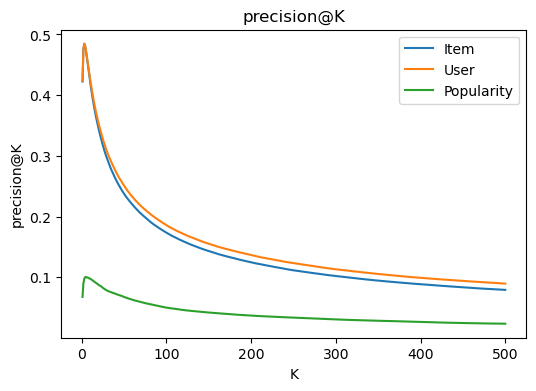
\includegraphics[width=\columnwidth]{precision-at-k.png}
\end{subfigure}
\caption{Average $precision\textrm{@}k$ for IB, UB, and popularity-based recommenders.}
\label{fig:precision-at-k}
\end{figure}

\section{Experimental Results}

In this section, we shall present the details of our experiments. The Kaggle
MSD Challenge dataset
contains a utility matrix $M_{\rm train}$ describing the
listening habit of all fully visible users in the trainset.
We are also given
$M^{\rm V}_{\rm test}$ and $M^{\rm H}_{\rm test}$, the
visible and hidden halves of the song history of the users in
$U_{\rm test}$\footnote{During the competition,
the contestants did not have access to $M^{\rm H}_{\rm test}$, but $M^{\rm H}_{\rm test}$ was
released afterwards for posterity. We evaluated our recommender only
after all hyper-parameter tuning was done.}.

We merged $M_{\rm train}$ and
$M^{\rm V}_{\rm test}$ into $M_{\rm all}$. Next, we randomly carved out $10\%$ of
the non-test users to form $U_{\rm valid}$,
and randomly hide half of these entries in the
utility matrix for the purpose of validation.
This methodology allows us to test and tune
our recommenders without peeking at the ground truth.
We then perform various experiments with different algorithms. The baseline
result is the popularity-based recommender, with an \mAP score
of only $2.3\%$.

\subsection{Neighborhood-based Recommenders}

Thanks in no small part to our architectural investment, we were able to
perform analysis on various combinations of hyper-parameters despite the tight
schedule. On average,
individual IB and UB runs took approximately $2$ to $3$ minutes each,

\begin{figure}[htbp]
\centering
\begin{subfigure}{0.85\columnwidth}
  \centering
  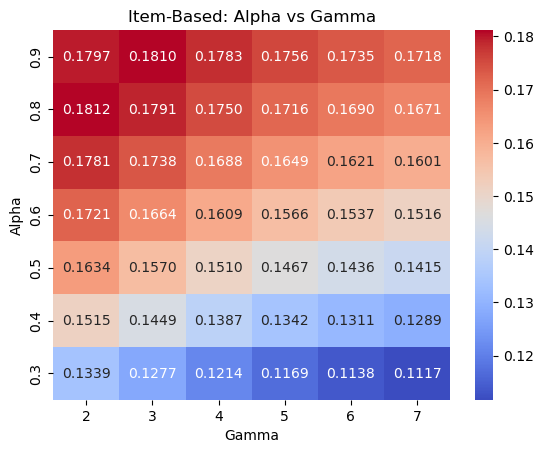
\includegraphics[width=\columnwidth]{item-grid-search.png}
\end{subfigure}
\caption{Grid Search on $\alpha$ and $\gamma$ for IB recommender.}
\label{fig:item-grid-search}
\end{figure}

\begin{figure}[htbp]
\centering
\begin{subfigure}{0.85\columnwidth}
  \centering
  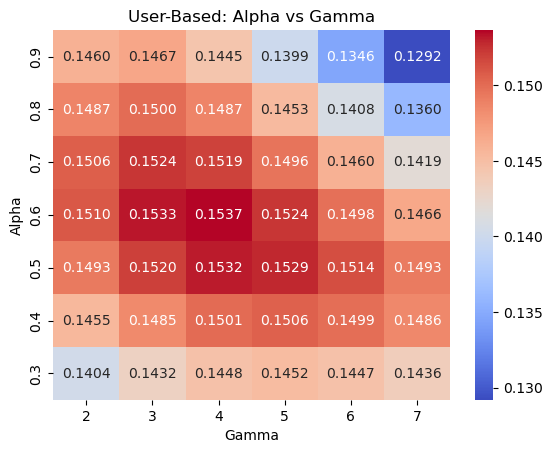
\includegraphics[width=\columnwidth]{user-grid-search.png}
\end{subfigure}
\caption{Grid Search on $\alpha$ and $\gamma$ for UB recommender.}
\label{fig:user-grid-search}
\end{figure}

$\alpha$ and $\gamma$ are
by far the most important hyper-parameters that determine
the performance of our IB and UB recommenders.
Figures~\ref{fig:item-grid-search} and \ref{fig:user-grid-search} show how
\mAP varies as a function of $\alpha$ and $\gamma$. We further
performed a local grid search around the hottest spots, and founded the
best parameters to be $\alpha_{\rm item} = 0.85$ and $\gamma_{\rm item} = 2.5$
for item-based recommender, and $\alpha_{user}=0.65$ and $\gamma_{user}=4.0$
for user-based recommender. The \mAP for the IB recommender alone is
$18.18\%$, and that for the UB recommender alone is $15.38\%$.

\subsection{Ensemble Recommender}

Our ensemble recommender has a tunable parameter $\rho$, which
modifies the weights of the input recommenders. In the experiment
shown in Figure~\ref{fig:rho-grid-search}, we made a recommendation based
on an IB recommender and a UB recommender, and varied $\rho$ between $0.25$
and $5.00$ inclusive. The weights for the two recommenders were simply
$0.18$ and $0.15$ respectively. The ensemble recommender outperforms
both IB and UB recommenders across all choices of $\rho$. At the best
value of $\rho$, the \mAP of the ensembler exceeds that of IB by $2.3\%$,
and that of UB by $20.9\%$.

\begin{figure}[htbp]
\centering
\begin{subfigure}{0.85\columnwidth}
  \centering
  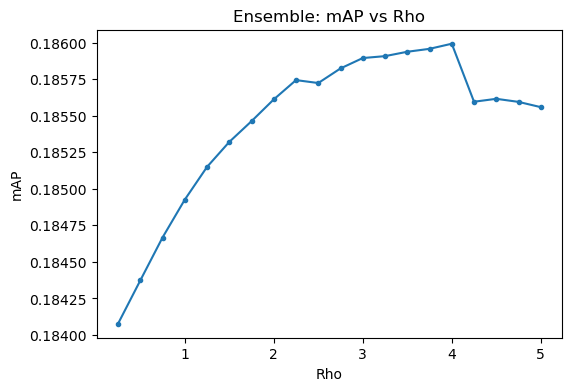
\includegraphics[width=\columnwidth]{rho-grid-search.png}
\end{subfigure}
\caption{Grid Search on $\rho$ for ensemble recommender.}
\label{fig:rho-grid-search}
\end{figure}

\subsection{Comparison on the Validation Set}

We now compare the \mAP and runtime performance of different algorithms.
Performance is measured with both the truncated \mAP metric evaluated at
$\tau=500$ (see \cite{Bertin-Mahieux2011}), and a
metric called coverage,
which simply measures the average percentage of songs in the
ground truth correctly predicted by the algorithm.
All experiments were performed on a single Quad-Core $2.33$GHz i$5$
Macbook Pro
circa $2018$ with $8$GB RAM, and all numbers quoted were measured with
a separate validation testset described earlier. \textsc{item-based} was
run with parameters $\alpha_{\rm item} = 0.85$ and $q_{\rm item} = 2.5$, and
\textsc{user-based} was
run with parameters $\alpha_{\rm item} = 0.65$ and $q_{\rm item} = 4.0$. The
complete \textsc{ensembler} algorithm utilized the output of these two 
recommenders, with $\rho = 4.0$. 
We also included both the raw runtime of \textsc{ensembler} and those of
\textsc{item-based} and \textsc{user-based}. All in all, \textsc{ensembler}
performed the best all other algorithms, achieving an \mAP score of
$18.599\%$.

The first and most obvious observation is the
poor performance of {\em all} embedding-based algorithms across
the board, whether it is from lyrics embeddings, matrix factorization
including \textsc{als} \cite{hu2008collaborative} and
\textsc{lmf} \cite{johnson2014logistic}, or using those embeddings in a
neighborhood-based setting. In fact, because of such poor performance, we
spent significant amount of time looking for bugs.

The second observation is that the ``\textsc{kiss}'' principle is readily
applicable. One would expect the more information we utilize, or the
more sophisticated the algorithms, the better result we would get. The
reality is more complicated. For example, we tried multiple ways to transform
the user-song-play triplets into more usable form, including
\textsc{tf-idf} and \textsc{bm-25}. At the end, a better understooding and
more elegant generalization of binary cosine similarity led to better
performance. In the case of the ensemble algorithm,
the more sophisticated and
theoretically sound ensembler $E_B$ lost out to the simpler ensembler $E_A$.

\begin{table*}[htbp]
\centering
\begin{tabular}{|c|c|c|c|c|c|}
\hline
\textsc{algorithm} & \textsc{parameters} & \textsc{mAP} & \textsc{coverage} & \textsc{wall runtime (sec)} & \textsc{cpu runtime {sec}} \\
\hline
\textsc{randomized} & & $0.001\%$ & $0.122\%$ & \tall $0$ \tall & $0$ \\
\textsc{embedding} & & $0.016\%$ & $0.666\%$ & \tall $4278$ \tall & $31331$ \\
\textsc{lmf}
\cite{johnson2014logistic} & & $1.586\%$ & $20.399\%$ & \tall $326$ \tall & $2302$ \\
\textsc{popularity} & & $2.354\%$ & $18.887\%$ & \tall $0$ \tall & $0$ \\
\textsc{als} \cite{hu2008collaborative} & & $4.671\%$ & $24.081\%$ & \tall $1391$ \tall & $9147$ \\
\textsc{user-based} (\textsc{UB}) & $\alpha(0.65),q(4.0)$ & $15.376\%$ & $49.007\%$ & \tall $159$ \tall & $1147$ \\
\textsc{item-based} (\textsc{IB}) & $\alpha(0.85),q(2.5)$ & $18.176\%$ & $57.546\%$ & \tall $116$ \tall & 815 \\
\hline
\textsc{ensembler} on (\textsc{IB}, \textsc{UB}) & $\rho(4.0)$ & $18.599\%$ & $58.385\%$ & \tall $13~(288)$ \tall & $13~(1975)$ \\
\hline
\end{tabular}
\vspace{1em}
\caption{Comparison among various algorithms. All runtimes exclude the
overhead of reading the input data and minor preprocessing. The \mAP metric
reports the truncated version at $\tau=500$ (see \cite{Bertin-Mahieux2011}).
The \textsc{coverage} metric measures the average percentage of songs in the
ground truth correctly predicted by the algorithm.
All numbers quoted were measured with
a validation test set randomly splitted from the training data.
The \textsc{ensembler} runtime
in parenthesis includes those of the item-based and user-based runtime.}
\label{table:performance}
\end{table*}

\subsection{A Moment of Truth with Kaggle}

Unfortuntately, despite the great performance of our ensemble algorithm,
it did not perform as well as we expected when we run it on the actual
testset. We achieved an \mAP score of
$17.453\%$, which is a significant drop from our best result of
$18.599\%$ evaluated on the validation set.
In retrospect, we realized we made a major mistake in not conducting
enough cross-validation during grid search, and
hence the result might have been somewhat overfitted. Sadly, we did not
have enough time to correct course. That said, the
\mAP score of $17.453\%$ would have placed our team in second place in the
Kaggle leaderboard, behind only the winner at $17.909\%$.

\section{Discussion}

While disappointing at first, we realized the goal of
the project has never been to achieve the top ranking. Instead, we gained
an appreciation for good architecture and implementation. 
On the other hand,
while it is possible that what we saw was the result of an extremely
embarrassing bug, we may have an explanation for 
the surprisingly poor performance
of embedding-based approaches.

Let's first take a detour to
revisit the Netflix Prize, in which the objective was to
minimize the RMSE of rating prediction. It would be three long years before
the winning team beat the prior art by $10\%$, achieving an RMSE of $0.8563$.
Since the lowest and highest movie ratings are $1$ and $5$ respectively,
the RMSE spans a whooping $\frac{0.8563}{5-1} \simeq 21.4\%$ of the ranges.
These RMSE represents a combination of inherent noise and uncertainty
that even the best recommender cannot overcome.

In the MSD Challenge, on the other hand,
the ability to correctly predict the items early
in the ranking would make or break the recommenders. Here lies an
important difference between RMSE (Netflix) and \mAP (MSDC): while RMSE
emphasizes on accuracy in an equitable fashion (accurate ratings on bad
movies are valued just as much as those on good movies),
\mAP focuses exclusively on
the very top rankings. In our dataset, the average number of items per user is
$\frac{|M|}{|U|} \simeq 48$, a miniscule number comparing to the $380K$
items. From this perspective, even the $2.3\%$ \mAP achieved by
the popularity-based recommender looks impressive!

But how come embedding-based recommenders perform so much worse
than IB and UB recommenders? The key may be the {\em quality} of the
similarity measures. In Figure~\ref{fig:similarity}, we took a snapshot of the
$sim(i,\star)$ vector each time we process a new item $i$, sorted them and
normalized them so the largest value is $1$. Afterwards, we sampled and
tallied each half-percentage between $0\%$ and $10\%$. In other words, we
are interested in the dropoff in the values of similarity across
all items. Notice how the similarity scores decrease at different rates.

We postulate that the structure of the neighborhood landscape, as measured
by similarity, plays a significant role in the accuracy of prediction.
It may not be very helpful to have too many similar items, just like it would
be annoying and unproductive to hear ``most anything is good here!'' when
asking the waitress to recommend a dish.
We have consistently observed that steeper curves
coincide with better \mAP performances. In fact, this would explain why
increasing the locality factor $\gamma$ improves performance, as
it is an inexpensive way to steepen the curve.
Perhaps this is why in the grid-search we found
$\gamma_{\rm user} > \gamma_{\rm item} > 1$.

\begin{figure}[htbp]
\centering
\begin{subfigure}{0.85\columnwidth}
  \centering
  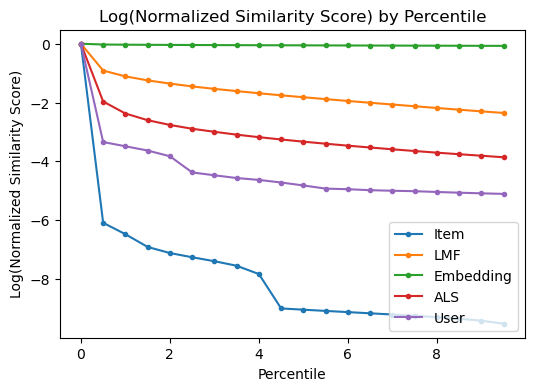
\includegraphics[width=\columnwidth]{similarity.png}
\end{subfigure}
\caption{Logarithm of normalized similarity score at each precision
point ($precision\textrm{@}k$) for each recommender.}
\label{fig:similarity}
\end{figure}

In conclusion, we have investigated the Million Song Dataset Challenge and
implemented multiple algorithms. Our solution was built on a robust, efficient,
and flexible architecture that allowed us to explore and fine-tune various
possibilities.

\section*{Appendix -- Work Assignment}

The initial intent was that all three members make equal
(or at least equitable) contributions towards the project.

We share research and background discovery equally
among Carlos, Hardy, and John.
A significant amount of time was spent on
nailing down the project choice and refinement.

Hardy was responsible for all C++ implementation including collaborative
filtering, ensembler, and the use of Python
Implicit (\textsc{als} and \textsc{lmf}). John was responsible
for the development of embedding assignment including a significant amount of
research on how to create useful embeddings from \textsc{Word2vec},
and \textsc{GloVe}. John also
looked into other topics related to embedding such as genre classification.

The report was written by Hardy, including various experiments that
accompanied the analysis (e.g.~Discussion section). John made the
presentation.

\bibliographystyle{acm}
\bibliography{report}

\end{document}
